%
\section{Nützliches und Wissenswertes zum Erstellen einer Seminarausarbeitung}
\label{sec_stil}

Kleiner genereller Abschnitt über unsere Methode.

\subsection{Data Sources}
\label{subsec_method_datasources}

\emph{Match Forrest, Match!} is built on four different data sources.

The first data source is the \textit{Internet Movie Database (IMDb)}\footnote{\url{http://www.imdb.com/}}.
This data source contains more than 274,000 movies and more than 365,000 people.
%TODO SOURCE ^
To get the individual movie resources, the system has to crawl HTML pages.
While the content in \textit{IMDb} is mostly user-generated, it has to go through multiple consistency checks, performed by professionals \cite{IMDb_DataCreation}.
Thus, we can assume that the data is more likely to be correct when compared to data from entirely user generated data sources.

Another big movie platform is \textit{Freebase}\footnote{\url{http://www.freebase.com/}}.
\textit{Freebase} is a connected user-generated open database, which contains a lot of links to other platforms.
It contains more than 250,000 movies and more than 430,000 people.
%TODO SOURCE ^
\textit{Freebase} offers a MQL API and a Topic API, which can be queried to get movie resources.

\textit{themoviedb.org (TMDb)}\footnote{\url{http://www.themoviedb.org/}} is a movie database which contains a lot of images.
It also offers an API to send requests for movie resources.
\textit{TMDb} is a collection of more than 171,000 movies and 605,000 people.
%TODO SOURCE ^
\textit{TMDb} also published diffs, which is helpful to keep all movies from this data source up-to-date.

The last data source the system utilizes is the \textit{Online-Filmdatenbank (OFDb)}\footnote{\url{http://www.ofdb.de/}}.
This data source is specialised on German movies, but also contains international ones.
It contains more than 236,000 movies and 54,000 people.
%TODO SOURCE ^
%TODO ??Table for the numbers instead??
\\ \\
To create a unified dataset of movies, a main data source must be chosen.
This main source is used to match movies from different data sources against it.
For \emph{Match Forrest, Match!} \textit{IMDb} was chosen as the main data source, since it contains more movies than any of the other data sources.
Additionally, \textit{IMDb} is maintained by data editors, which manually add, delete and update the data\footnote{\url{https://uk-amazon.icims.com/jobs/274286/data-editor\%2c-database-content/job}}.

All the other data sources are not maintained by paid professionals or are not as big as \textit{IMDb}.
\\ \\
Some movies from \textit{Freebase}, \textit{TMDb} and \textit{OFDb} already contain links to the correpsonding \textit{IMDb} movie.
This is immensely helpful in the matching process (Chapter \ref{subsec_method_matching}).
%!TEX root = ../../lod-group1.tex
\subsection{Movie Ontology}
\label{subsec_method_ontology}

As described in the previous section, different data sources, each having their own data format, were used in the system \emph{Match Forrest, Match!}.
To create a unified dataset and therefore enable simple querying over all data, an ontology for movies was defined.

This ontology covers movie resources as well as resources which belong to a movie, such as awards.
In general, the defined ontology is based on the DBpedia ontology.
If no DBpedia class or property was present, Freebase classes or properties or newly defined ones were used.

In the following, the defined entities used in the system with their corresponding RDF classes are listed in Table \ref{tab_entities}.

\begin{table}[ht]
	\begin{center}
	\begin{tabular}{ll}
		\textbf{Entity} & \textbf{RDF class} \\ \hline
		Movie & dbpedia-owl:Film \\
		Award & dbpedia-owl:Award \\
		MoviePerson & dbpedia-owl:Person \\
		Character & freebase:film/performance \\
		MovieCharacter & lod:MovieCharacter \\
		Aka (also known as) & lod:Aka \\
		ReleaseInfo & lod:ReleaseInfo \\
	\end{tabular}
	\end{center}
	\caption{Entities with their corresponding RDF classes}
	\label{tab_entities}
\end{table}

Relations between these resources and their pattern for the unique identifiers are shown in Figure \ref{fig_ontology}.
The prefix \textit{lod} was newly defined for this project.

\begin{figure}[h!]
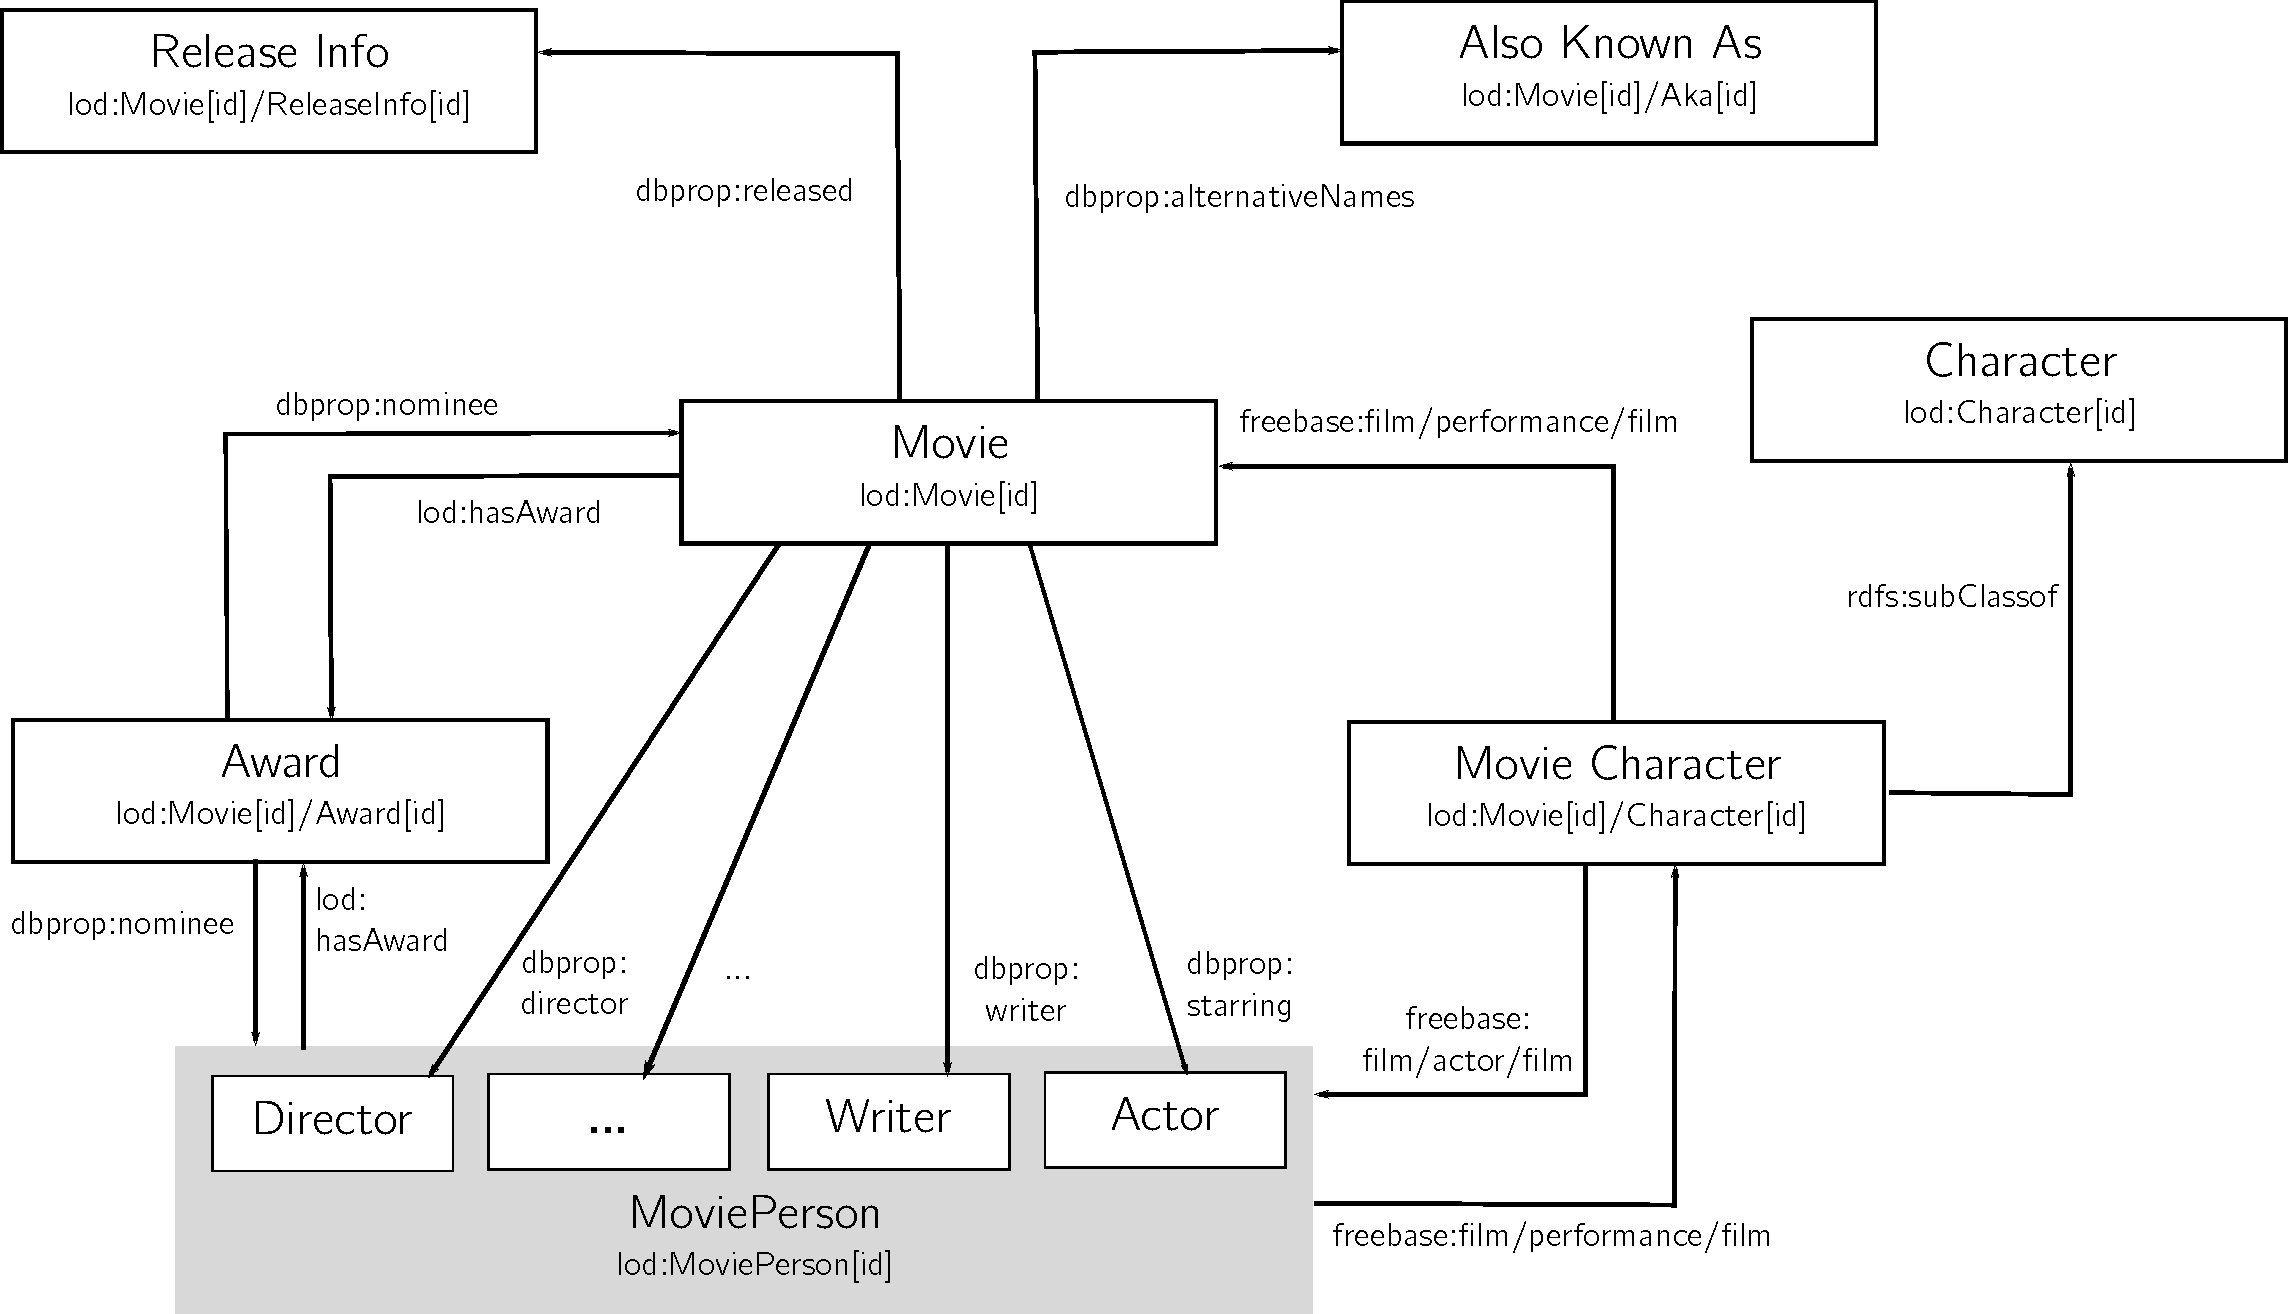
\includegraphics[width=\textwidth]{images/ontology.pdf}
\caption{Movie Ontology. Relations between all resources and their pattern for the unique identifiers.}
\label{fig_ontology}
\end{figure}

A MoviePerson can have multiple sub-types of \textit{dbpedia-owl:Person}, depending on the jobs the person had on any movies they worked on.
As shown in Figure \ref{fig_ontology} a distinction between these jobs (e.g. director, writer, producer) was made.
For example, a person who is a director in one movie and an actor in another movie would have the additional classes \textit{dbpedia-owl:Actor} and \textit{dbpedia-owl:Director}.

A problem, which occured when defining our ontology, was the entity Character.
In the initial definition, there was just one character class, which was connected to the corresponding movie and actor.
The actor also had a connection to the character.
The unique identifier of the character was build from the character's name.

Thus, a character which exists in multiple movies (e.g. "cleaning lady") would be one resource connected to each actor who had ever portrayed this character.
The character also had a list of movies which it occured in.
That way, one could not say which actors played the character in a certain movie.
One such case is an actor who played a certain character in an old movie but also appears in the movie's newer remake.
In the remake, they might play a different character while another actor plays their original character.
An example for this is the movie "Starsky \& Hutch" (2004), which is a remake of the 1970s television series with the same name.
In the movie, both actors which originally portrayed Starsky and Hutch get a cameo appearance alongside the new cast for their old characters.
With the old approach, the system could not know who played the Starsky character in the remake, because all actors who ever played the character are listed.

Therefore, an additional class of MovieCharacter was introduced in the final ontology.
This resource is only connected to one movie and all actors, who played that character in that movie.
The unique identifier of the MovieCharacter is build from the unique identifier of the movie and the character.
The MovieCharacter is a subclass of Character, which describes the general character.
This means, that the unique identifier of the MovieCharacter in the "Starsky \& Hutch" example is "Starksy/Starsky\&Hutch1970" and identifier of Character is "Starksy".
\subsection{Triplification}
\label{subsec_method_triplification}
\subsection{Matching}
\label{subsec_method_matching}

The following sections show the approach for matching (i.e. finding the same entity in different datasets) and merging (i.e. integrating two different datasets about the same entity into one.)

\subsubsection{Problem statement}
After loading the initial dataset into the database, the task is to integrate another dataset to finally create a whole dataset with more information than a single one can provide on their own.
% TODO: Why IMDB?
However, simply dumping the second dataset into the database would lead to duplicated entries and thereby decreasing the overall quality of the database.
Thus, the datasets need to be aggregated and unified.
Matching movies, actors, ... but now focus on movies. TODO

A first approach is to match movies by their name.
However, only using the name as a matching criteria yields multiple problems, such as:
\begin{itemize}
	\item different movies having the same name e.g.
	\begin{itemize} 
        \item The Avengers (2012) vs. The Avengers (1998)
    \end{itemize}
	\item same movies having different names in different datasets e.g.
	\begin{itemize} 
        \item typos: Batman vs Badman
        \item localization: The Internship vs. Prakti.com
        \item formating: The Italian Job vs. Italian Job, The
     \end{itemize}
\end{itemize}
Hence, a more sophisticated approach needs to be developed to increase the quality of the dataset.

\subsubsection{Matching using Actor overlap}
In general, the matching algorithm must satisfy two requirements:
\begin{enumerate}
	\item{High precision}: A movies should not be matched to a wrong movie.
	\item{Performance:} Matching should not take to long TODO
\end{enumerate}

The former 
General idea: actor overlap

\paragraph{Candidate selection}

\paragraph{Score calculation}

\subsubsection{Refinement}
\subsection{Updating}
\label{subsec_method_updating}

To ensure that the movies are always up to date, a scheduler is responsible to update the movies at certain, repeading times.
The scheduler downloads movie resources, which should be updated, triplifies them and stores them into the triple store.
Thereby, the schedule distinguish between existing movies - movies, which are released in the past from the current date - and coming soon movies - movies, which are resleased in the future.

\subsubsection{Updating coming soon movies}
Upcoming movies are published almost every day on IMDB (Chapter \ref{subsec_evaluation_updating}).
Because IMDB is the main data source, the scheduler updates upcoming movies from IMDB daily.
Upcoming movies from the other data sources are updated weekly.
In this way, movies, which come from freebase, TMDB or OFDB, can already be matched to a movie of IMDB.

The steps to update upcoming soon movies are:
\begin {enumerate}
	\item Get new movie resources with their ids.
	\item For each movie, download the new movie resource and triplify it.
	\item Delete all triples of the movie in the triple store in the corresponding graph, if the movie already exists.
	\item Load triples of an IMDB movie into the corresponding graph in the triple store. For the other resources, integrate  the triples of the upcoming movie and store them in the corresponding graph.
\end{enumerate}

To get all new movies from IMDB, the scheduler crawls the "Coming Soon" page (\url{http://www.imdb.com/movies-coming-soon/2014-08/}) from the current month until the same month next year.
This page contains all new movies ids, which will be released in the time period crawled.
Having the new movie ids, the scheduler automatically has the new movie resource, which can be crawled.

Freebase has an API, which the scheduler ask for all movies ids.
Afterwards, the scheduler filters the ids for those ids, which are unknown.

% TODO
% TMDB
% Get all ids higher than the last id
% OFDB
% Get all ids higher than the last id

\subsubsection{Updating existing movies}
Existings movies are divided into different categories.
Each category is updated at different frequencies (Table \ref{tab_updating_existing}).
\begin{table}[h]
	\caption{Frequency of updating existing movies}
	\begin{center}
	\begin{tabular}{rl}
		\textbf{category of movie} & \textbf{frequency} \\ \hline
		one year old & weekly \\
		5 year old & monthly \\
		5 - 25 years old & yearly \\
		older than 25 years & never \\
	\end{tabular}
	\end{center}
	\label{tab_updating_existing}
\end{table}
If a category should be updated, the scheduler does the follwing steps:
\begin{enumerate}
	\item Find all movies, which should be updated regardless their originial data source.
	\item For each of these movies, get the updated movie resource and triplify it.
	\item Delete all triples of the movie in the triple store in the corresponding graph.
	\item Load the new triples into the corresponding graph in the triple store.
\end{enumerate}
Because the movies are stored in different graphs depending on their originial data source, the scheduler knows, where to find the movie resource in the web.
The originial resource of a movie is stored in a \emph{sameAs} triple to the movie.
Deleting the existing triples and storing the new downloaded triples, ensures that no conflicting information is stored of a resource.
\subsection{Architecture}
\label{subsec_method_architecture}

\begin{figure}[ht]
  \begin{center}
  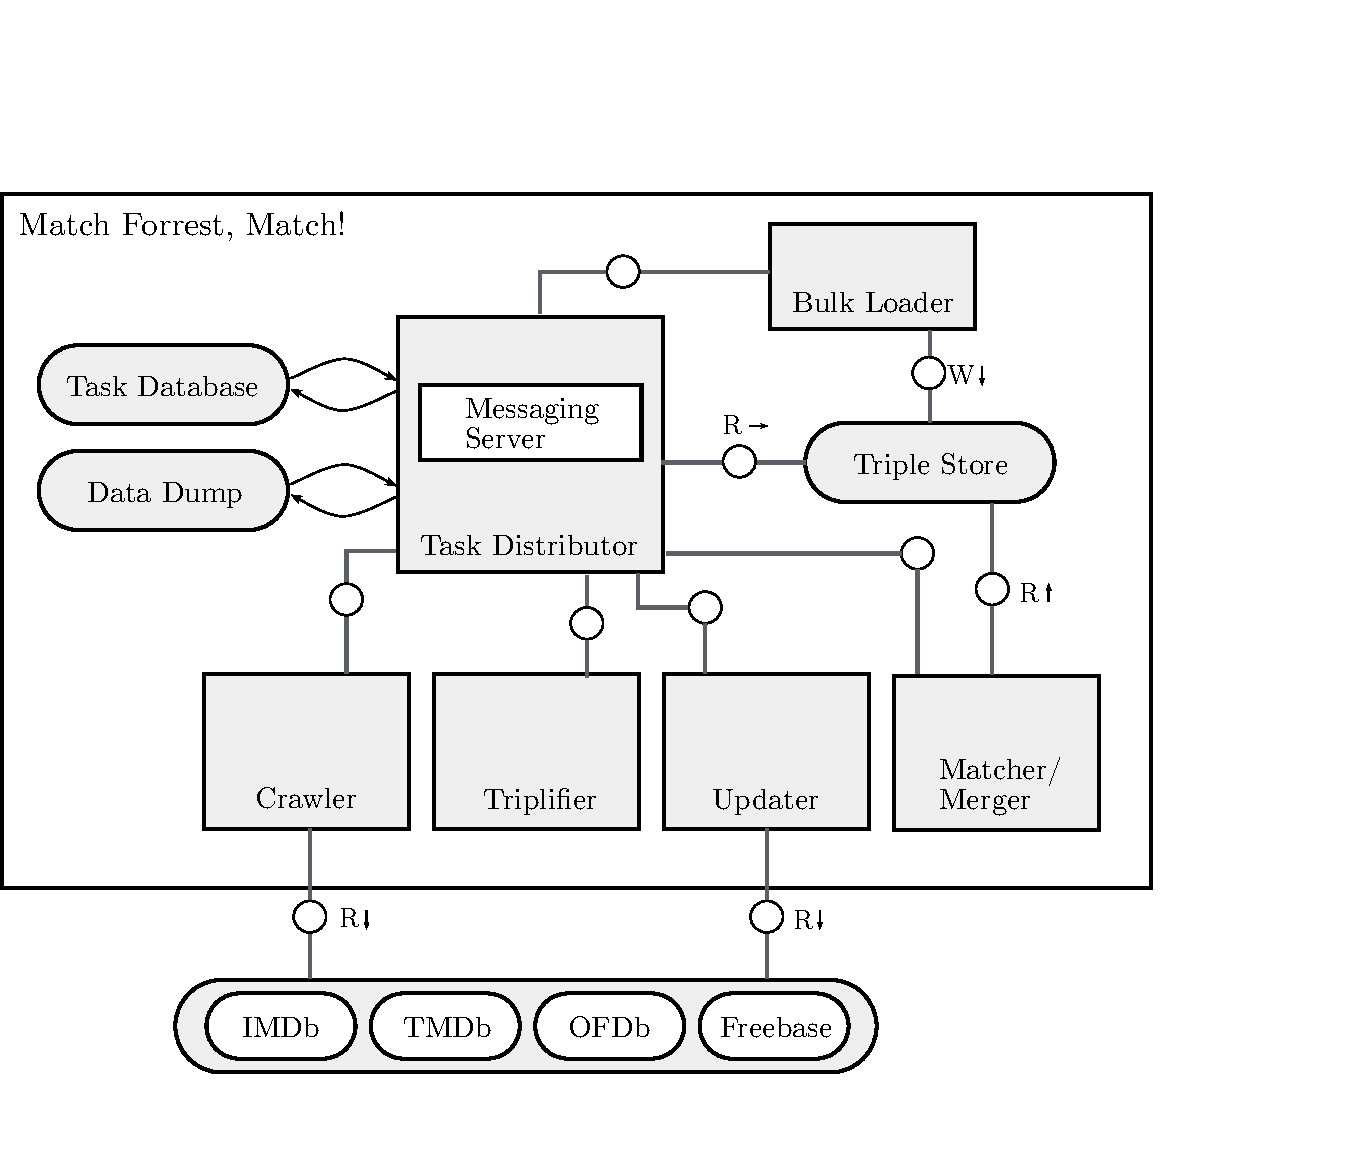
\includegraphics[width=0.5\textwidth]{images/architecture.pdf}
  \end{center}
  \caption{Architecture}
  \label{fig_architecture}
\end{figure}

\subsubsection{Messaging Infrastructure}
\label{subsubsec_messaging_infrastructure}

\begin{figure}[ht]
  \begin{center}
  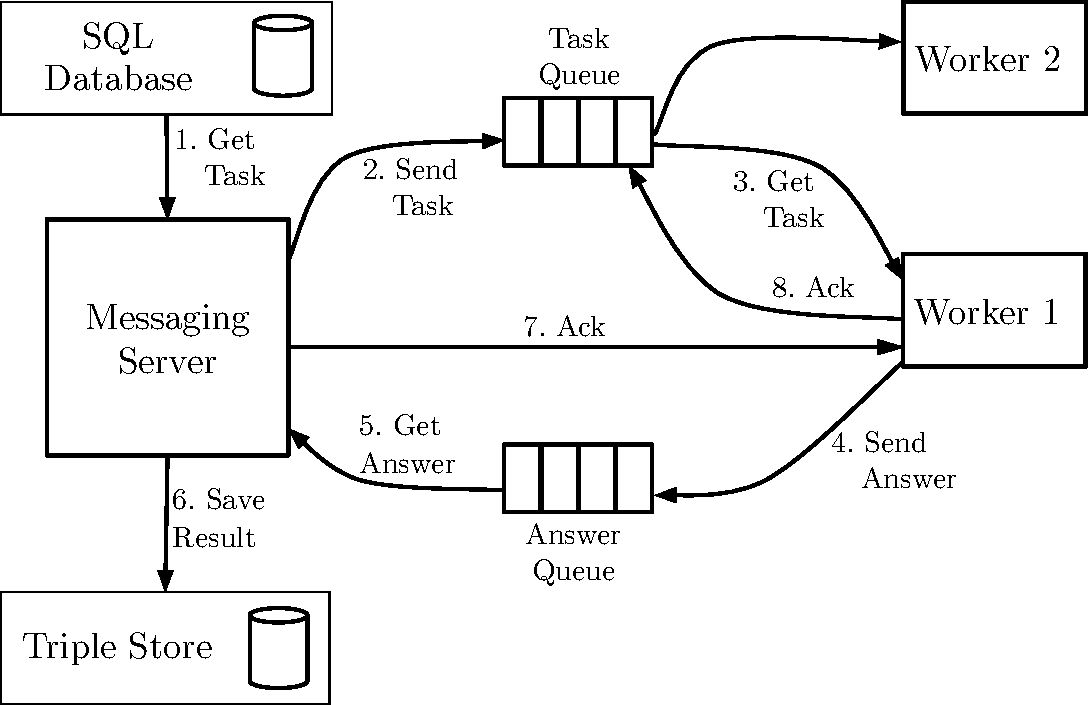
\includegraphics[width=0.5\textwidth]{images/rabbit_mq.pdf}
  \end{center}
  \caption{Messaging Infrastructure using RabbitMQ}
  \label{fig_messaging_infrastructure}
\end{figure}


\subsection{Allgemeine Hinweise}
Ganz allgemein handelt es sich bei der Seminarausarbeitung bereits um eine {\bf wissenschaftliche Arbeit}.
Begehen Sie nicht den Fehler und sehen Sie diese als wortwörtliche Wiedergabe Ihres Seminarvortrags an, sondern beachten Sie stets die folgenden Punkte:
\begin{itemize}
\item Die sprachliche Darstellung sollte dem Rahmen angepasst sein und stets auf einer sachlichen Argumentationsebene rangieren.
\item Der Schreibstil sollte unpersönlich gehalten werden.
Vermeiden Sie Sätze, die die Wörter "`wir"', "`uns"', "`Sie"' usw.~enthalten.\footnote{Eine Ausnahme von dieser Regel stellen persönliche Kommentare, Bewertungen oder Urteile von Sachverhalten dar. Hier sollte klar werden, dass es sich um Ihre eigene Leistung handelt.}
\item Vermeiden Sie (Bandwurm-)Sätze\index{Bandwurmsatz}, die sich über mehr als 2--3 Zeilen ziehen. Sie erhöhen damit signifikant die Lesbarkeit Ihrer Arbeit.
\item Vermeiden Sie sprachliche Komplexität, d.h. beschränken Sie die Anzahl der notwendigen Nebensätze auf ein Mindestmaß.
\item Drücken Sie sich einfach und präzise aus. Vermeiden Sie eine \glqq geschraubte\grqq\, Ausdrucksweise.
\item Achten Sie auf temporale Konsistenz in der Verwendung von Präsens\index{Präsens} oder Präteritum \index{Präteritum} bei Verben.
\item Vermeiden Sie Worthülsen\index{Worthülsen} und unnötige Redewendungen ohne signifikanten Inhalt.
\item Legen Sie Ihren Standpunkt stets mit der angemessenen Objektivität dar, auch wenn es um die Bewertung von Vor- oder Nachteilen des jeweiligen Themengegenstandes geht.
\item Vermeiden Sie unnötige Anglizismen\index{Anglizismen} (z.B.~"`connecten, downloaden, backupen"').
Existiert in diesem Zusammenhang bereits eine deutsche Redewendung, dann benutzen Sie diese (z.B. "`öffentlicher Schlüssel"' statt "`public key"').
Verwenden Sie englische Begriffe, so passen Sie diese entsprechend den deutschen Rechtschreibregeln bez.~Flexion, Silbentrennung, Getrennt- und Zusammenschreibung an.
\item Wenn Sie Begriffe einführen bzw. verwenden, deren Bedeutung nicht unmittelbar auch einem Nichtfachmann geläufig ist, sollten diese stets erläutert werden.
Die Fachbegriffe sollten unmittelbar im Text oder im Text {\bf und} dem Glossar erklärt werden.
In natur- und. ingenieurwissenschaftlichen Arbeiten ist es eher unüblich, Erklärungen in Fußnoten zu platzieren.
\item Achten Sie auf einen {\bf logischen Aufbau} Ihrer Arbeit, sowie ihrer einzelnen Unterkapitel und Gliederungspunkte.
\item {\bf Dringende Empfehlung:} Lassen Sie Ihre Ausarbeitung am besten von einem "`Nichtfachmann"'/einer "`Nichtfachfrau"', also nicht von einem Informatiker/einer Informatikerin Korrekturlesen.
Auf diese Weise werden Schwachstellen in Ihrer Argumentation und andere logische Mängel am deutlichsten.
\item Verwenden Sie konsequent die {\bf neue deutsche Rechtschreibung}\index{Rechtschreibung}.
Lassen Sie Ihren Text von einem Rechtschreibprogramm prüfen.
Allerdings kann dieses nur die korrekte Schreibweise von Einzelwörtern und nicht die korrekte Verwendung von Einzelwörtern im Satzzusammenhang überprüfen, insbesondere wenn es um grammatikalische Fehler\index{Grammatikfehler} oder Kommasetzung\index{Kommasetzung} geht.
Verlassen Sie sich daher nicht alleine auf das Programm.
\item In deutschen Texten werden anstelle der englischen ''Quotes''\index{Quotes} die Anführungsstriche\index{Anführungsstriche} in Form von "`Gänsefüßchen"' geschrieben.
In dem Textsatzsystem {\LaTeX} stehen hierfür z.B. die Befehle \verb|\glqq| und \verb|\grqq| zur Verfügung. \\
{\bf Achtung:} Dazu muss das Paket {\tt ngerman}\index{ngerman} in den Header eingebunden werden.
\end{itemize}



\subsection{Weitere Formatierungshinweise}
\subsubsection{Abbildungen}
Abbildungen sind für das Erläutern und Verdeutlichen von komplexen Strukturen und Abläufen, wie sie üblicherweise in wissenschaftlichen Arbeiten beschrieben werden, unverzichtbar.
Die Abbildungen\index{Abbildung} in Ihrer Arbeit sind stets zu {\bf nummerieren} und wie folgt zu setzen (siehe Abb.~\ref{fig_Abb1}).
%Hier eine Abbildung
\begin{figure}[ht]
  \begin{center}
  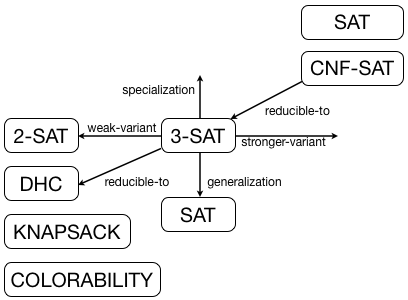
\includegraphics[width=0.5\textwidth]{images/3sat.pdf}
  \end{center}
  \caption{Das Umfeld des 3-SAT Problems}
  \label{fig_Abb1}
\end{figure}

Jede Abbildung soll neben einer Abbildungsnummer\index{Abbildung!Abbildungsnummer} eine Bildunterschrift\index{Abbildung!Bildunterschrift} ("`Das Umfeld des 3-SAT Problems"') besitzen, die die Grafik näher erläutert.
Weiterhin ist darauf zu achten, dass zu jeder Abbildung eine Bezugnahme im Text aufgenommen wird, d.h. an geeigneter Stelle sollte ein Verweis\index{Verweis} der Form (siehe Abb.~\dots) erfolgen.

Beachten Sie bitte, dass es sich bei der vorliegenden Grafik um eine .eps-Datei handelt (Encapsulated Postscript)\index{Encapsulated Postscript}, die mit Hilfe des \LaTeX-Pakets {\tt epsfig}\index{\LaTeX!epsfig} eingebunden wurde.
Die Abbildung kann natürlich auch mit Hilfe anderer Pakete eingebunden werden.
Achten Sie dabei aber stets auf eine für den Druck geeignete Bildqualität!

\smallskip

\begin{center}
\colorbox{lightgray}{
\parbox{140mm}{
{\bf Achtung:} \\
Eine Abbildung sollte nicht einfach per "`copy and paste"'\index{copy and paste} aus dem WWW\index{WWW} in Ihre Ausarbeitung übernommen werden.
Einerseits leidet im Allgemeinen bei einer solchen Vorgehensweise die Qualität\index{Abbildung!Bildqualität} bei einer entsprechenden Vergrößerung für die Druckaufbereitung\index{Abbildung!Druckaufbereitung} stark darunter (siehe Abb.~\ref{fig_Abb2}), anderseits muss sichergestellt werden, dass der Urheber der Originalgrafik damit einverstanden ist, dass die Grafik in die Seminararbeit aufgenommen wird.
Der sicherste Weg ist deshalb, die Grafik mit einem geeigneten Grafikprogramm {\em selbst} zu erzeugen und anschließend in den Text einzubinden.}}
\end{center}

%Hier eine Abbildung
\begin{figure}[ht]
  \begin{center}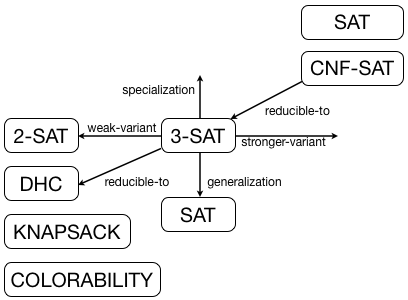
\includegraphics[width=0.5\textwidth]{images/3sat.png}\end{center}
  \caption{So sollte eine Abbildung nicht aussehen (JPG-Grafik, "`copy and paste"')}
  \label{fig_Abb2}
\end{figure}
Verwenden Sie eine Abbildung, die in dieser Form bzw. in einer sehr ähnlichen Form bereits veröffentlicht wurde, müssen Sie dies durch eine bibliografische Referenz deutlich machen, d.h. Sie müssen wie bei einem Zitat die Fundstelle im Text als Literaturangabe aufnehmen.



\subsubsection{Tabellen}
Für Tabellen\index{Tabelle} gilt dasselbe wie für Abbildungen.
Setzen Sie Tabellen nie in den Fließtext\index{Fließtext}, sondern in die entsprechende \LaTeX-Tabellenumgebung und versehen Sie diese ebenfalls mit einer {\em Tabellennummer}\index{Tabelle!Nummerierung} und einer Tabellen{\em überschrift}\index{Tabelle!Überschrift} (siehe Tabelle \ref{tab_HistoryWWW}).

%Hier eine Tabelle
\begin{table}
\caption{Die Geschichte des World Wide Web}
\begin{tabular}{rp{12cm}} \noalign{\smallskip} \hline \noalign{\smallskip}
{\bf 1945} & Vennevar Bush\index{Bush, Vennevar} beschreibt MEMEX\index{MEMEX}: das erste Hypertextsystem.\\
{\bf 1965} & Ted Nelson\index{Nelson, Ted} prägt als erster das Wort {\bf Hypertext}\index{Hypertext} auf der ACM-Jahreskonferenz.\\
{\bf 1968} & Doug Engelbart\index{Englebart, Douglas C.} entwickelt ein Hypertext-basiertes Prototypensystem NLS und erfindet zu diesem Zweck die Maus als Eingabegerät.\\
{\bf 1980} & Tim Berners Lee\index{Lee, Tim Berners} schreibt ein erste Notizbuch-Programm mit Hypertextlinks.\\
{\bf 1989} & Tim Berners Lee verfasst ein erstes Memorandum zu seinem Hypertext-Dokumentenverwaltungssystem am Kernforschungszentrum CERN.\\
{\bf 1990} & Zusammen mit Robert Cailliau\index{Cailliau, Robert} entwickelt Tim Berners Lee den ersten WWW-Server\index{Server} und WWW-Browser\index{Browser}: die Geburtsstunde des WorldWideWeb.\\  \noalign{\smallskip} \hline
\end{tabular}
\label{tab_HistoryWWW}
\end{table}

\noindent
Grundsätzlich sollte man bei dem Setzen einer Tabelle sparsam mit grafischen Elementen -- wie Hilfslinien oder bunte Tabellenunterlegungen -- umgehen, da diese die Lesbarkeit\index{Tabelle!grafische Gestaltung} sehr stark beeinträchtigen können.


\subsubsection{Listings, Quellcode und Pseudocode}

Sollten Sie Quellcode eines Programmes mit in Ihre Arbeit aufnehmen oder einen Algorithmus mit Hilfe von Pseudocode veranschaulichen, sind diese im Sinne einer Abbildung (siehe Abb.~\ref{fig_Abb3}) zu behandeln.
Ebenso wie eine Abbildung sind Listings\index{Listings}, Quellcode\index{Quellcode} oder Pseudocode\index{Pseudocode} jeweils mit einer laufenden Nummer und einer Bildunterschrift zu versehen.

\begin{figure}[ht]
\lstset{language=c++}
\lstset{backgroundcolor=\color{lightgray}}
\begin{lstlisting}{}
    for( i = 0; i < 10; i++ )
    {
        for( j = 0; j < 10; j++ )
        {
            // calculate $a_{ij}$
            a[i][j] = b[j][i];
        }
    }

\end{lstlisting}
  \caption{Einbinden von Quellcode in die Arbeit}
  \label{fig_Abb3}
\end{figure}

Sie können Listings z.B. mit Hilfe des \LaTeX-Pakets {\tt listings}\index{\LaTeX!listings} einbinden.
Insbesondere, wenn längere Quellcode-Passagen in den Text eingebunden werden sollen, empfiehlt sich diese Vorgehensweise, da das Paket automatisch Seitenumbrüche\index{Seitenumbruch} korrekt formatiert und auch die Verwendung von internen Zeilennummern\index{Zeilennummern} ermöglicht.

\subsubsection{Mathematische Formeln}\index{Formelsatz}

{\LaTeX} bietet sich insbesondere als Textverarbeitungssystem an, wenn es um das korrekte Formatieren mathematischer Ausdrücke und Formeln geht.
Versehen Sie alle Formeln, die Sie in Ihrer Arbeit verwenden -- insbesondere diejenigen, auf die Sie später noch Bezug nehmen --  mit einer entsprechenden Nummerierung.

\begin{equation}\label{formel1}
\frac{\sum_{n > 0} z^n}
{\prod_{1\leq k\leq n} (1-q^k)}
\end{equation}


\subsubsection{{\LaTeX} und andere Textverarbeitungssysteme}
Wenn Sie das Textsatzsystem {\LaTeX}\index{\LaTeX} für die Erstellung der Ausarbeitung verwenden, dann benutzen Sie das vorliegende \LaTeX-Musterdokument\index{\LaTeX!Musterdokument} als Layoutvorlage für Ihre Arbeit.
Sollten Sie ein anderes Textverarbeitungsprogramm als {\LaTeX} verwenden, dann halten Sie sich bitte an die in diesem Beispieldokument verwendeten Bemaßungen und Formatierungen.
Sie können sich z.B.~dieses Beipieldokument ausdrucken und die entsprechenden Maßangaben, wie
\begin{itemize}
\item linker, rechter Rand
\item Abstand oben, unten
\item etc.
\end{itemize}
abmessen und in Ihrem eigenen Textverarbeitungsprogramm verwenden. \\
Denken Sie bitte daran, dass neben einer gedruckten Version Ihrer Seminarausarbeitung auch eine {\bf pdf}-Datei\index{pdf} abzugeben ist.
Diese können Sie zusammen mit Ihrer Präsentation (pdf-Datei + evtl.~ppt-Datei) via E-Mail zusenden.
